\documentclass{standalone}
\usepackage{tikz}
\begin{document}
    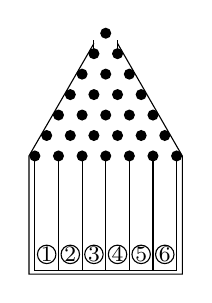
\begin{tikzpicture}
      \tikzset{mynode/.style={draw,circle,minimum size=0pt,inner sep=0pt,font=\footnotesize}}
        \foreach \x in{0,0.3,0.6,...,2.1}
        \fill[] (240:\x)circle(2pt) ;

        \foreach\y/\z in{0.3/1.8,0.6/1.5,0.9/1.2,1.2/0.9}
       { \begin{scope}[shift={(300:\y)}]
          \foreach \x in{0,0.3,...,\z} 
          \fill[]  (240:\x)circle(2pt) ;
        \end{scope} }

        \begin{scope}[shift={(300:1.5)}]
           \foreach \x in {0,0.3}
            \fill[]  (240:\x)circle(2pt) ;
          \end{scope}
         \begin{scope}[shift={(300:1.8)}]
            
             \fill[]  (240:0)circle(2pt) ;
           \end{scope}
       \draw[] ([yshift=0.17cm]240:0.3)--++(0,-5pt);
       \draw[] ([yshift=0.17cm]300:0.3)--++(0,-5pt);
       \draw[] ([yshift=3.7pt]240:0.3)--++(240:1.65)--++(0,-1.5)--++(1.8cm+4.2pt,0)--++(0,1.5)--([yshift=3.7pt]300:0.3);

       \draw[] (240:1.8)--++(0,-1.45)--++(1.8,0)--++(0,1.45);
       \foreach \x in{0.3,0.6,...,1.8}
       \draw[] (240:1.8)+(\x,0)--++(\x,-1.45);
       \foreach \x/\y in{0.15/1,0.45/2,0.75/3,1.05/4,1.35/5,1.65/6}
       \node[]  at ([shift={(\x,-1.25)}]240:1.8) {\tikz\node[mynode] at (0,0){\y};}; 
      
    \end{tikzpicture}
\end{document}